\begin{figure}[H] \centering % Created by tikzDevice version 0.12.4 on 2023-07-16 16:33:32
% !TEX encoding = UTF-8 Unicode
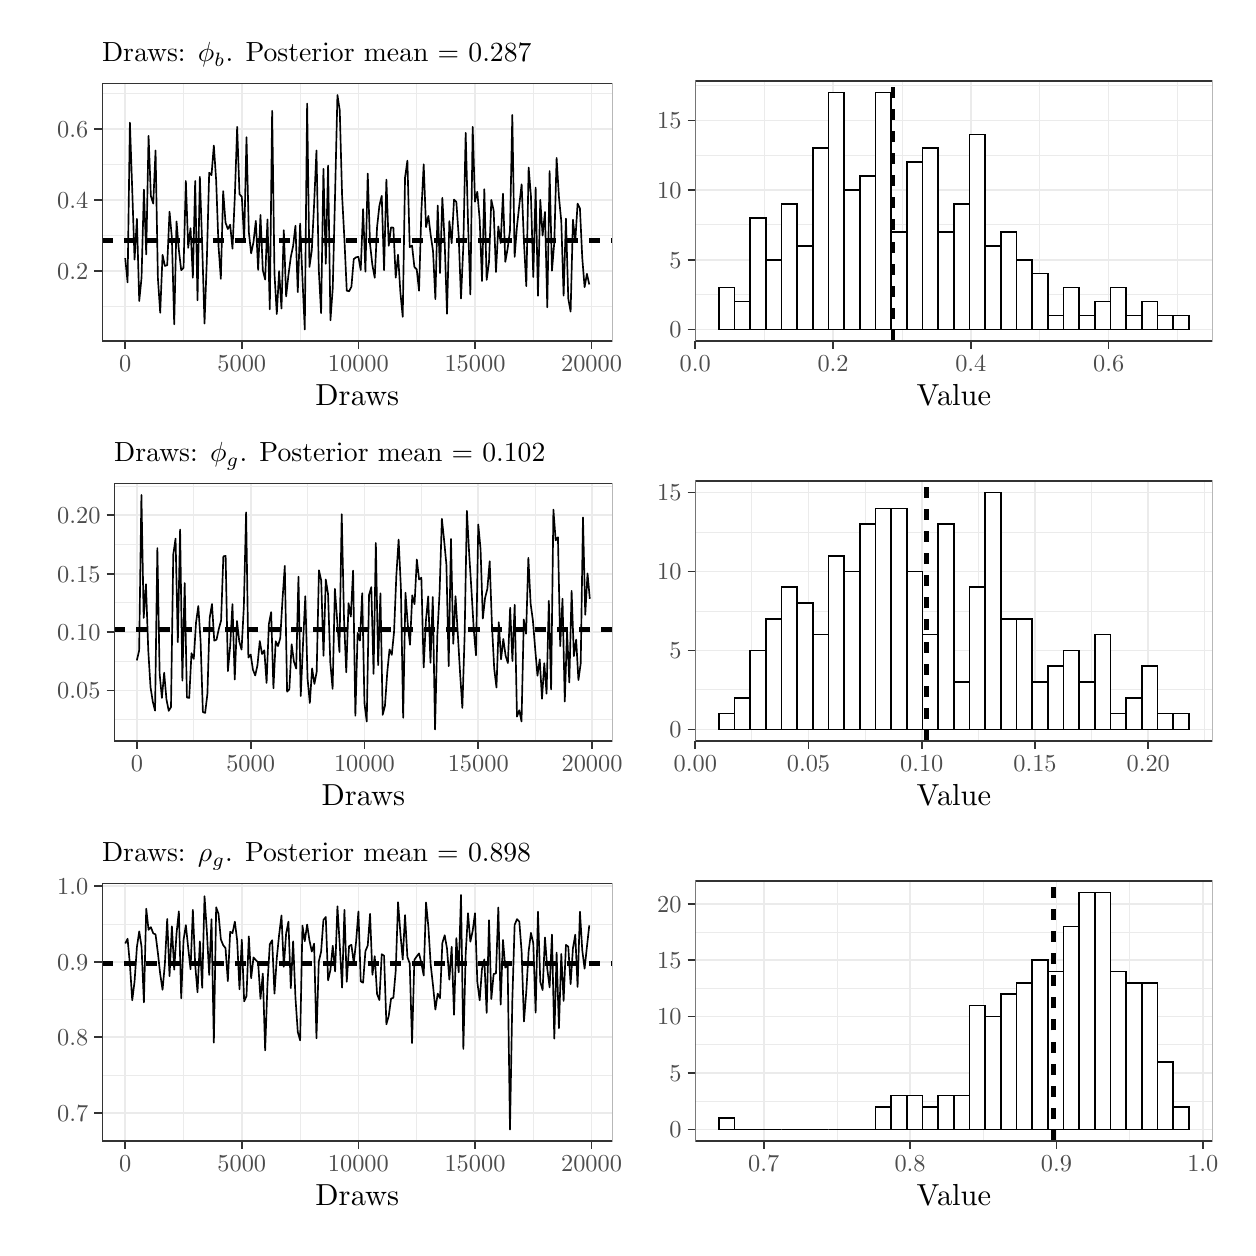
\begin{tikzpicture}[x=1pt,y=1pt]
\definecolor{fillColor}{RGB}{255,255,255}
\path[use as bounding box,fill=fillColor,fill opacity=0.00] (0,0) rectangle (433.62,433.62);
\begin{scope}
\path[clip] (  0.00,289.08) rectangle (216.81,433.62);
\definecolor{drawColor}{RGB}{255,255,255}
\definecolor{fillColor}{RGB}{255,255,255}

\path[draw=drawColor,line width= 0.6pt,line join=round,line cap=round,fill=fillColor] (  0.00,289.08) rectangle (216.81,433.62);
\end{scope}
\begin{scope}
\path[clip] ( 26.87,320.33) rectangle (211.31,413.52);
\definecolor{fillColor}{RGB}{255,255,255}

\path[fill=fillColor] ( 26.87,320.33) rectangle (211.31,413.52);
\definecolor{drawColor}{gray}{0.92}

\path[draw=drawColor,line width= 0.3pt,line join=round] ( 26.87,332.76) --
	(211.31,332.76);

\path[draw=drawColor,line width= 0.3pt,line join=round] ( 26.87,358.44) --
	(211.31,358.44);

\path[draw=drawColor,line width= 0.3pt,line join=round] ( 26.87,384.13) --
	(211.31,384.13);

\path[draw=drawColor,line width= 0.3pt,line join=round] ( 26.87,409.81) --
	(211.31,409.81);

\path[draw=drawColor,line width= 0.3pt,line join=round] ( 56.32,320.33) --
	( 56.32,413.52);

\path[draw=drawColor,line width= 0.3pt,line join=round] ( 98.45,320.33) --
	( 98.45,413.52);

\path[draw=drawColor,line width= 0.3pt,line join=round] (140.58,320.33) --
	(140.58,413.52);

\path[draw=drawColor,line width= 0.3pt,line join=round] (182.70,320.33) --
	(182.70,413.52);

\path[draw=drawColor,line width= 0.6pt,line join=round] ( 26.87,345.60) --
	(211.31,345.60);

\path[draw=drawColor,line width= 0.6pt,line join=round] ( 26.87,371.29) --
	(211.31,371.29);

\path[draw=drawColor,line width= 0.6pt,line join=round] ( 26.87,396.97) --
	(211.31,396.97);

\path[draw=drawColor,line width= 0.6pt,line join=round] ( 35.25,320.33) --
	( 35.25,413.52);

\path[draw=drawColor,line width= 0.6pt,line join=round] ( 77.38,320.33) --
	( 77.38,413.52);

\path[draw=drawColor,line width= 0.6pt,line join=round] (119.51,320.33) --
	(119.51,413.52);

\path[draw=drawColor,line width= 0.6pt,line join=round] (161.64,320.33) --
	(161.64,413.52);

\path[draw=drawColor,line width= 0.6pt,line join=round] (203.77,320.33) --
	(203.77,413.52);
\definecolor{drawColor}{RGB}{0,0,0}

\path[draw=drawColor,line width= 0.6pt,line join=round] ( 35.25,350.34) --
	( 36.10,341.59) --
	( 36.94,399.29) --
	( 37.78,375.06) --
	( 38.62,349.79) --
	( 39.47,364.52) --
	( 40.31,334.84) --
	( 41.15,343.32) --
	( 42.00,375.10) --
	( 42.84,351.68) --
	( 43.68,394.52) --
	( 44.52,372.79) --
	( 45.37,370.04) --
	( 46.21,389.25) --
	( 47.05,343.20) --
	( 47.89,330.60) --
	( 48.74,351.53) --
	( 49.58,347.54) --
	( 50.42,347.76) --
	( 51.26,367.10) --
	( 52.11,357.70) --
	( 52.95,326.42) --
	( 53.79,363.62) --
	( 54.63,353.27) --
	( 55.48,345.98) --
	( 56.32,346.82) --
	( 57.16,378.22) --
	( 58.00,354.05) --
	( 58.85,361.16) --
	( 59.69,343.24) --
	( 60.53,378.24) --
	( 61.37,335.11) --
	( 62.22,379.71) --
	( 63.06,355.05) --
	( 63.90,326.70) --
	( 64.74,349.66) --
	( 65.59,381.21) --
	( 66.43,380.33) --
	( 67.27,391.03) --
	( 68.11,378.40) --
	( 68.96,354.76) --
	( 69.80,342.86) --
	( 70.64,374.56) --
	( 71.49,363.19) --
	( 72.33,360.85) --
	( 73.17,362.40) --
	( 74.01,353.76) --
	( 74.86,372.75) --
	( 75.70,397.78) --
	( 76.54,373.47) --
	( 77.38,372.50) --
	( 78.23,356.89) --
	( 79.07,394.06) --
	( 79.91,359.82) --
	( 80.75,352.06) --
	( 81.60,356.14) --
	( 82.44,363.81) --
	( 83.28,346.06) --
	( 84.12,365.91) --
	( 84.97,345.94) --
	( 85.81,342.60) --
	( 86.65,364.32) --
	( 87.49,331.84) --
	( 88.34,403.58) --
	( 89.18,344.79) --
	( 90.02,330.16) --
	( 90.86,345.66) --
	( 91.71,332.10) --
	( 92.55,360.45) --
	( 93.39,336.48) --
	( 94.23,344.28) --
	( 95.08,350.73) --
	( 95.92,354.74) --
	( 96.76,362.05) --
	( 97.60,338.05) --
	( 98.45,362.79) --
	( 99.29,342.93) --
	(100.13,324.57) --
	(100.98,406.20) --
	(101.82,347.16) --
	(102.66,353.06) --
	(103.50,369.75) --
	(104.35,389.22) --
	(105.19,346.21) --
	(106.03,330.47) --
	(106.87,382.61) --
	(107.72,348.29) --
	(108.56,383.81) --
	(109.40,327.88) --
	(110.24,339.51) --
	(111.09,373.84) --
	(111.93,409.29) --
	(112.77,403.73) --
	(113.61,373.10) --
	(114.46,356.96) --
	(115.30,338.57) --
	(116.14,338.36) --
	(116.98,339.98) --
	(117.83,350.00) --
	(118.67,350.63) --
	(119.51,350.80) --
	(120.35,346.06) --
	(121.20,368.03) --
	(122.04,345.42) --
	(122.88,380.89) --
	(123.72,355.34) --
	(124.57,347.77) --
	(125.41,343.26) --
	(126.25,361.50) --
	(127.09,369.28) --
	(127.94,372.84) --
	(128.78,345.99) --
	(129.62,378.72) --
	(130.47,354.78) --
	(131.31,361.42) --
	(132.15,361.36) --
	(132.99,343.28) --
	(133.84,351.58) --
	(134.68,337.93) --
	(135.52,329.11) --
	(136.36,379.45) --
	(137.21,385.56) --
	(138.05,354.32) --
	(138.89,354.90) --
	(139.73,347.16) --
	(140.58,346.28) --
	(141.42,338.56) --
	(142.26,367.16) --
	(143.10,384.24) --
	(143.95,361.53) --
	(144.79,365.57) --
	(145.63,358.68) --
	(146.47,352.90) --
	(147.32,335.55) --
	(148.16,369.34) --
	(149.00,344.97) --
	(149.84,372.15) --
	(150.69,355.92) --
	(151.53,330.21) --
	(152.37,363.72) --
	(153.21,355.77) --
	(154.06,371.49) --
	(154.90,370.63) --
	(155.74,358.41) --
	(156.58,335.72) --
	(157.43,354.93) --
	(158.27,395.61) --
	(159.11,363.54) --
	(159.96,337.19) --
	(160.80,397.78) --
	(161.64,370.74) --
	(162.48,374.32) --
	(163.33,364.17) --
	(164.17,342.08) --
	(165.01,375.24) --
	(165.85,342.48) --
	(166.70,348.90) --
	(167.54,371.37) --
	(168.38,367.56) --
	(169.22,345.35) --
	(170.07,361.80) --
	(170.91,355.81) --
	(171.75,373.61) --
	(172.59,348.99) --
	(173.44,353.83) --
	(174.28,360.29) --
	(175.12,402.07) --
	(175.96,350.79) --
	(176.81,361.85) --
	(177.65,369.48) --
	(178.49,377.02) --
	(179.33,356.10) --
	(180.18,340.22) --
	(181.02,383.09) --
	(181.86,372.73) --
	(182.70,343.48) --
	(183.55,375.86) --
	(184.39,336.74) --
	(185.23,371.40) --
	(186.07,358.51) --
	(186.92,367.02) --
	(187.76,332.60) --
	(188.60,381.80) --
	(189.45,345.80) --
	(190.29,356.04) --
	(191.13,386.54) --
	(191.97,372.44) --
	(192.82,363.65) --
	(193.66,336.79) --
	(194.50,364.63) --
	(195.34,335.75) --
	(196.19,331.01) --
	(197.03,364.22) --
	(197.87,356.44) --
	(198.71,370.03) --
	(199.56,368.29) --
	(200.40,350.45) --
	(201.24,339.84) --
	(202.08,344.67) --
	(202.93,340.82);

\path[draw=drawColor,line width= 1.7pt,dash pattern=on 4pt off 4pt ,line join=round] ( 26.87,356.77) -- (211.31,356.77);
\definecolor{drawColor}{gray}{0.20}

\path[draw=drawColor,line width= 0.6pt,line join=round,line cap=round] ( 26.87,320.33) rectangle (211.31,413.52);
\end{scope}
\begin{scope}
\path[clip] (  0.00,  0.00) rectangle (433.62,433.62);
\definecolor{drawColor}{gray}{0.30}

\node[text=drawColor,anchor=base east,inner sep=0pt, outer sep=0pt, scale=  0.88] at ( 21.92,342.57) {0.2};

\node[text=drawColor,anchor=base east,inner sep=0pt, outer sep=0pt, scale=  0.88] at ( 21.92,368.26) {0.4};

\node[text=drawColor,anchor=base east,inner sep=0pt, outer sep=0pt, scale=  0.88] at ( 21.92,393.94) {0.6};
\end{scope}
\begin{scope}
\path[clip] (  0.00,  0.00) rectangle (433.62,433.62);
\definecolor{drawColor}{gray}{0.20}

\path[draw=drawColor,line width= 0.6pt,line join=round] ( 24.12,345.60) --
	( 26.87,345.60);

\path[draw=drawColor,line width= 0.6pt,line join=round] ( 24.12,371.29) --
	( 26.87,371.29);

\path[draw=drawColor,line width= 0.6pt,line join=round] ( 24.12,396.97) --
	( 26.87,396.97);
\end{scope}
\begin{scope}
\path[clip] (  0.00,  0.00) rectangle (433.62,433.62);
\definecolor{drawColor}{gray}{0.20}

\path[draw=drawColor,line width= 0.6pt,line join=round] ( 35.25,317.58) --
	( 35.25,320.33);

\path[draw=drawColor,line width= 0.6pt,line join=round] ( 77.38,317.58) --
	( 77.38,320.33);

\path[draw=drawColor,line width= 0.6pt,line join=round] (119.51,317.58) --
	(119.51,320.33);

\path[draw=drawColor,line width= 0.6pt,line join=round] (161.64,317.58) --
	(161.64,320.33);

\path[draw=drawColor,line width= 0.6pt,line join=round] (203.77,317.58) --
	(203.77,320.33);
\end{scope}
\begin{scope}
\path[clip] (  0.00,  0.00) rectangle (433.62,433.62);
\definecolor{drawColor}{gray}{0.30}

\node[text=drawColor,anchor=base,inner sep=0pt, outer sep=0pt, scale=  0.88] at ( 35.25,309.32) {0};

\node[text=drawColor,anchor=base,inner sep=0pt, outer sep=0pt, scale=  0.88] at ( 77.38,309.32) {5000};

\node[text=drawColor,anchor=base,inner sep=0pt, outer sep=0pt, scale=  0.88] at (119.51,309.32) {10000};

\node[text=drawColor,anchor=base,inner sep=0pt, outer sep=0pt, scale=  0.88] at (161.64,309.32) {15000};

\node[text=drawColor,anchor=base,inner sep=0pt, outer sep=0pt, scale=  0.88] at (203.77,309.32) {20000};
\end{scope}
\begin{scope}
\path[clip] (  0.00,  0.00) rectangle (433.62,433.62);
\definecolor{drawColor}{RGB}{0,0,0}

\node[text=drawColor,anchor=base,inner sep=0pt, outer sep=0pt, scale=  1.10] at (119.09,297.01) {Draws};
\end{scope}
\begin{scope}
\path[clip] (  0.00,  0.00) rectangle (433.62,433.62);
\definecolor{drawColor}{RGB}{0,0,0}

\node[text=drawColor,anchor=base west,inner sep=0pt, outer sep=0pt, scale=  1.00] at ( 26.87,421.23) {Draws: $\phi_b$. Posterior mean = 0.287};
\end{scope}
\begin{scope}
\path[clip] (216.81,289.08) rectangle (433.62,433.62);
\definecolor{drawColor}{RGB}{255,255,255}
\definecolor{fillColor}{RGB}{255,255,255}

\path[draw=drawColor,line width= 0.6pt,line join=round,line cap=round,fill=fillColor] (216.81,289.08) rectangle (433.62,433.62);
\end{scope}
\begin{scope}
\path[clip] (241.24,320.33) rectangle (428.12,414.43);
\definecolor{fillColor}{RGB}{255,255,255}

\path[fill=fillColor] (241.24,320.33) rectangle (428.12,414.43);
\definecolor{drawColor}{gray}{0.92}

\path[draw=drawColor,line width= 0.3pt,line join=round] (241.24,337.19) --
	(428.12,337.19);

\path[draw=drawColor,line width= 0.3pt,line join=round] (241.24,362.35) --
	(428.12,362.35);

\path[draw=drawColor,line width= 0.3pt,line join=round] (241.24,387.51) --
	(428.12,387.51);

\path[draw=drawColor,line width= 0.3pt,line join=round] (241.24,412.67) --
	(428.12,412.67);

\path[draw=drawColor,line width= 0.3pt,line join=round] (266.13,320.33) --
	(266.13,414.43);

\path[draw=drawColor,line width= 0.3pt,line join=round] (315.92,320.33) --
	(315.92,414.43);

\path[draw=drawColor,line width= 0.3pt,line join=round] (365.72,320.33) --
	(365.72,414.43);

\path[draw=drawColor,line width= 0.3pt,line join=round] (415.51,320.33) --
	(415.51,414.43);

\path[draw=drawColor,line width= 0.6pt,line join=round] (241.24,324.61) --
	(428.12,324.61);

\path[draw=drawColor,line width= 0.6pt,line join=round] (241.24,349.77) --
	(428.12,349.77);

\path[draw=drawColor,line width= 0.6pt,line join=round] (241.24,374.93) --
	(428.12,374.93);

\path[draw=drawColor,line width= 0.6pt,line join=round] (241.24,400.09) --
	(428.12,400.09);

\path[draw=drawColor,line width= 0.6pt,line join=round] (241.24,320.33) --
	(241.24,414.43);

\path[draw=drawColor,line width= 0.6pt,line join=round] (291.03,320.33) --
	(291.03,414.43);

\path[draw=drawColor,line width= 0.6pt,line join=round] (340.82,320.33) --
	(340.82,414.43);

\path[draw=drawColor,line width= 0.6pt,line join=round] (390.61,320.33) --
	(390.61,414.43);
\definecolor{drawColor}{RGB}{0,0,0}

\path[draw=drawColor,line width= 0.6pt,fill=fillColor] (249.73,324.61) rectangle (255.39,339.71);

\path[draw=drawColor,line width= 0.6pt,fill=fillColor] (255.39,324.61) rectangle (261.06,334.67);

\path[draw=drawColor,line width= 0.6pt,fill=fillColor] (261.06,324.61) rectangle (266.72,364.87);

\path[draw=drawColor,line width= 0.6pt,fill=fillColor] (266.72,324.61) rectangle (272.38,349.77);

\path[draw=drawColor,line width= 0.6pt,fill=fillColor] (272.38,324.61) rectangle (278.05,369.90);

\path[draw=drawColor,line width= 0.6pt,fill=fillColor] (278.05,324.61) rectangle (283.71,354.80);

\path[draw=drawColor,line width= 0.6pt,fill=fillColor] (283.71,324.61) rectangle (289.37,390.03);

\path[draw=drawColor,line width= 0.6pt,fill=fillColor] (289.37,324.61) rectangle (295.04,410.16);

\path[draw=drawColor,line width= 0.6pt,fill=fillColor] (295.04,324.61) rectangle (300.70,374.93);

\path[draw=drawColor,line width= 0.6pt,fill=fillColor] (300.70,324.61) rectangle (306.36,379.96);

\path[draw=drawColor,line width= 0.6pt,fill=fillColor] (306.36,324.61) rectangle (312.03,410.16);

\path[draw=drawColor,line width= 0.6pt,fill=fillColor] (312.03,324.61) rectangle (317.69,359.84);

\path[draw=drawColor,line width= 0.6pt,fill=fillColor] (317.69,324.61) rectangle (323.35,385.00);

\path[draw=drawColor,line width= 0.6pt,fill=fillColor] (323.35,324.61) rectangle (329.02,390.03);

\path[draw=drawColor,line width= 0.6pt,fill=fillColor] (329.02,324.61) rectangle (334.68,359.84);

\path[draw=drawColor,line width= 0.6pt,fill=fillColor] (334.68,324.61) rectangle (340.34,369.90);

\path[draw=drawColor,line width= 0.6pt,fill=fillColor] (340.34,324.61) rectangle (346.00,395.06);

\path[draw=drawColor,line width= 0.6pt,fill=fillColor] (346.00,324.61) rectangle (351.67,354.80);

\path[draw=drawColor,line width= 0.6pt,fill=fillColor] (351.67,324.61) rectangle (357.33,359.84);

\path[draw=drawColor,line width= 0.6pt,fill=fillColor] (357.33,324.61) rectangle (362.99,349.77);

\path[draw=drawColor,line width= 0.6pt,fill=fillColor] (362.99,324.61) rectangle (368.66,344.74);

\path[draw=drawColor,line width= 0.6pt,fill=fillColor] (368.66,324.61) rectangle (374.32,329.64);

\path[draw=drawColor,line width= 0.6pt,fill=fillColor] (374.32,324.61) rectangle (379.98,339.71);

\path[draw=drawColor,line width= 0.6pt,fill=fillColor] (379.98,324.61) rectangle (385.65,329.64);

\path[draw=drawColor,line width= 0.6pt,fill=fillColor] (385.65,324.61) rectangle (391.31,334.67);

\path[draw=drawColor,line width= 0.6pt,fill=fillColor] (391.31,324.61) rectangle (396.97,339.71);

\path[draw=drawColor,line width= 0.6pt,fill=fillColor] (396.97,324.61) rectangle (402.64,329.64);

\path[draw=drawColor,line width= 0.6pt,fill=fillColor] (402.64,324.61) rectangle (408.30,334.67);

\path[draw=drawColor,line width= 0.6pt,fill=fillColor] (408.30,324.61) rectangle (413.96,329.64);

\path[draw=drawColor,line width= 0.6pt,fill=fillColor] (413.96,324.61) rectangle (419.63,329.64);

\path[draw=drawColor,line width= 1.7pt,dash pattern=on 4pt off 4pt ,line join=round] (312.69,320.33) -- (312.69,414.43);
\definecolor{drawColor}{gray}{0.20}

\path[draw=drawColor,line width= 0.6pt,line join=round,line cap=round] (241.24,320.33) rectangle (428.12,414.43);
\end{scope}
\begin{scope}
\path[clip] (  0.00,  0.00) rectangle (433.62,433.62);
\definecolor{drawColor}{gray}{0.30}

\node[text=drawColor,anchor=base east,inner sep=0pt, outer sep=0pt, scale=  0.88] at (236.29,321.58) {0};

\node[text=drawColor,anchor=base east,inner sep=0pt, outer sep=0pt, scale=  0.88] at (236.29,346.74) {5};

\node[text=drawColor,anchor=base east,inner sep=0pt, outer sep=0pt, scale=  0.88] at (236.29,371.90) {10};

\node[text=drawColor,anchor=base east,inner sep=0pt, outer sep=0pt, scale=  0.88] at (236.29,397.06) {15};
\end{scope}
\begin{scope}
\path[clip] (  0.00,  0.00) rectangle (433.62,433.62);
\definecolor{drawColor}{gray}{0.20}

\path[draw=drawColor,line width= 0.6pt,line join=round] (238.49,324.61) --
	(241.24,324.61);

\path[draw=drawColor,line width= 0.6pt,line join=round] (238.49,349.77) --
	(241.24,349.77);

\path[draw=drawColor,line width= 0.6pt,line join=round] (238.49,374.93) --
	(241.24,374.93);

\path[draw=drawColor,line width= 0.6pt,line join=round] (238.49,400.09) --
	(241.24,400.09);
\end{scope}
\begin{scope}
\path[clip] (  0.00,  0.00) rectangle (433.62,433.62);
\definecolor{drawColor}{gray}{0.20}

\path[draw=drawColor,line width= 0.6pt,line join=round] (241.24,317.58) --
	(241.24,320.33);

\path[draw=drawColor,line width= 0.6pt,line join=round] (291.03,317.58) --
	(291.03,320.33);

\path[draw=drawColor,line width= 0.6pt,line join=round] (340.82,317.58) --
	(340.82,320.33);

\path[draw=drawColor,line width= 0.6pt,line join=round] (390.61,317.58) --
	(390.61,320.33);
\end{scope}
\begin{scope}
\path[clip] (  0.00,  0.00) rectangle (433.62,433.62);
\definecolor{drawColor}{gray}{0.30}

\node[text=drawColor,anchor=base,inner sep=0pt, outer sep=0pt, scale=  0.88] at (241.24,309.32) {0.0};

\node[text=drawColor,anchor=base,inner sep=0pt, outer sep=0pt, scale=  0.88] at (291.03,309.32) {0.2};

\node[text=drawColor,anchor=base,inner sep=0pt, outer sep=0pt, scale=  0.88] at (340.82,309.32) {0.4};

\node[text=drawColor,anchor=base,inner sep=0pt, outer sep=0pt, scale=  0.88] at (390.61,309.32) {0.6};
\end{scope}
\begin{scope}
\path[clip] (  0.00,  0.00) rectangle (433.62,433.62);
\definecolor{drawColor}{RGB}{0,0,0}

\node[text=drawColor,anchor=base,inner sep=0pt, outer sep=0pt, scale=  1.10] at (334.68,297.01) {Value};
\end{scope}
\begin{scope}
\path[clip] (  0.00,144.54) rectangle (216.81,289.08);
\definecolor{drawColor}{RGB}{255,255,255}
\definecolor{fillColor}{RGB}{255,255,255}

\path[draw=drawColor,line width= 0.6pt,line join=round,line cap=round,fill=fillColor] (  0.00,144.54) rectangle (216.81,289.08);
\end{scope}
\begin{scope}
\path[clip] ( 31.27,175.79) rectangle (211.31,268.98);
\definecolor{fillColor}{RGB}{255,255,255}

\path[fill=fillColor] ( 31.27,175.79) rectangle (211.31,268.98);
\definecolor{drawColor}{gray}{0.92}

\path[draw=drawColor,line width= 0.3pt,line join=round] ( 31.27,183.55) --
	(211.31,183.55);

\path[draw=drawColor,line width= 0.3pt,line join=round] ( 31.27,204.66) --
	(211.31,204.66);

\path[draw=drawColor,line width= 0.3pt,line join=round] ( 31.27,225.76) --
	(211.31,225.76);

\path[draw=drawColor,line width= 0.3pt,line join=round] ( 31.27,246.87) --
	(211.31,246.87);

\path[draw=drawColor,line width= 0.3pt,line join=round] ( 31.27,267.98) --
	(211.31,267.98);

\path[draw=drawColor,line width= 0.3pt,line join=round] ( 60.02,175.79) --
	( 60.02,268.98);

\path[draw=drawColor,line width= 0.3pt,line join=round] (101.14,175.79) --
	(101.14,268.98);

\path[draw=drawColor,line width= 0.3pt,line join=round] (142.26,175.79) --
	(142.26,268.98);

\path[draw=drawColor,line width= 0.3pt,line join=round] (183.39,175.79) --
	(183.39,268.98);

\path[draw=drawColor,line width= 0.6pt,line join=round] ( 31.27,194.10) --
	(211.31,194.10);

\path[draw=drawColor,line width= 0.6pt,line join=round] ( 31.27,215.21) --
	(211.31,215.21);

\path[draw=drawColor,line width= 0.6pt,line join=round] ( 31.27,236.32) --
	(211.31,236.32);

\path[draw=drawColor,line width= 0.6pt,line join=round] ( 31.27,257.43) --
	(211.31,257.43);

\path[draw=drawColor,line width= 0.6pt,line join=round] ( 39.45,175.79) --
	( 39.45,268.98);

\path[draw=drawColor,line width= 0.6pt,line join=round] ( 80.58,175.79) --
	( 80.58,268.98);

\path[draw=drawColor,line width= 0.6pt,line join=round] (121.70,175.79) --
	(121.70,268.98);

\path[draw=drawColor,line width= 0.6pt,line join=round] (162.82,175.79) --
	(162.82,268.98);

\path[draw=drawColor,line width= 0.6pt,line join=round] (203.95,175.79) --
	(203.95,268.98);
\definecolor{drawColor}{RGB}{0,0,0}

\path[draw=drawColor,line width= 0.6pt,line join=round] ( 39.45,204.98) --
	( 40.28,208.56) --
	( 41.10,264.75) --
	( 41.92,220.33) --
	( 42.74,232.48) --
	( 43.57,208.71) --
	( 44.39,195.31) --
	( 45.21,190.08) --
	( 46.03,186.84) --
	( 46.86,245.54) --
	( 47.68,200.24) --
	( 48.50,191.40) --
	( 49.32,200.52) --
	( 50.15,190.84) --
	( 50.97,186.77) --
	( 51.79,188.11) --
	( 52.61,243.26) --
	( 53.44,248.99) --
	( 54.26,211.59) --
	( 55.08,252.27) --
	( 55.90,197.64) --
	( 56.73,232.94) --
	( 57.55,191.57) --
	( 58.37,191.42) --
	( 59.19,207.58) --
	( 60.02,205.54) --
	( 60.84,218.70) --
	( 61.66,224.62) --
	( 62.48,211.99) --
	( 63.31,186.33) --
	( 64.13,186.00) --
	( 64.95,192.94) --
	( 65.77,220.37) --
	( 66.60,225.34) --
	( 67.42,212.10) --
	( 68.24,212.49) --
	( 69.06,216.32) --
	( 69.89,219.39) --
	( 70.71,242.58) --
	( 71.53,242.73) --
	( 72.35,201.09) --
	( 73.17,210.14) --
	( 74.00,225.32) --
	( 74.82,198.08) --
	( 75.64,219.19) --
	( 76.46,211.83) --
	( 77.29,208.86) --
	( 78.11,224.31) --
	( 78.93,258.48) --
	( 79.75,206.01) --
	( 80.58,207.09) --
	( 81.40,201.61) --
	( 82.22,199.55) --
	( 83.04,203.27) --
	( 83.87,211.96) --
	( 84.69,207.28) --
	( 85.51,208.63) --
	( 86.33,196.82) --
	( 87.16,218.15) --
	( 87.98,222.42) --
	( 88.80,194.90) --
	( 89.62,211.90) --
	( 90.45,210.17) --
	( 91.27,213.03) --
	( 92.09,227.09) --
	( 92.91,239.14) --
	( 93.74,193.69) --
	( 94.56,194.56) --
	( 95.38,210.82) --
	( 96.20,204.64) --
	( 97.03,202.01) --
	( 97.85,235.24) --
	( 98.67,192.11) --
	( 99.49,210.91) --
	(100.32,228.18) --
	(101.14,198.32) --
	(101.96,189.59) --
	(102.78,202.08) --
	(103.61,196.48) --
	(104.43,200.84) --
	(105.25,237.54) --
	(106.07,233.83) --
	(106.90,206.63) --
	(107.72,234.21) --
	(108.54,228.96) --
	(109.36,204.12) --
	(110.19,194.71) --
	(111.01,230.85) --
	(111.83,219.53) --
	(112.65,208.02) --
	(113.48,257.84) --
	(114.30,220.23) --
	(115.12,200.68) --
	(115.94,225.64) --
	(116.77,220.80) --
	(117.59,237.43) --
	(118.41,184.97) --
	(119.23,214.90) --
	(120.06,212.13) --
	(120.88,229.27) --
	(121.70,189.47) --
	(122.52,182.90) --
	(123.35,228.61) --
	(124.17,231.44) --
	(124.99,200.11) --
	(125.81,247.41) --
	(126.64,203.26) --
	(127.46,229.22) --
	(128.28,185.31) --
	(129.10,188.57) --
	(129.93,200.62) --
	(130.75,208.93) --
	(131.57,206.99) --
	(132.39,215.30) --
	(133.22,235.70) --
	(134.04,248.65) --
	(134.86,231.30) --
	(135.68,184.25) --
	(136.51,229.43) --
	(137.33,218.21) --
	(138.15,210.61) --
	(138.97,228.49) --
	(139.80,225.31) --
	(140.62,241.44) --
	(141.44,234.21) --
	(142.26,234.86) --
	(143.09,202.42) --
	(143.91,219.39) --
	(144.73,228.12) --
	(145.55,204.15) --
	(146.38,227.87) --
	(147.20,180.03) --
	(148.02,213.91) --
	(148.84,229.56) --
	(149.67,256.17) --
	(150.49,248.27) --
	(151.31,239.54) --
	(152.13,202.91) --
	(152.96,248.84) --
	(153.78,210.95) --
	(154.60,228.16) --
	(155.42,214.65) --
	(156.25,200.42) --
	(157.07,187.79) --
	(157.89,213.94) --
	(158.71,258.99) --
	(159.54,243.45) --
	(160.36,230.39) --
	(161.18,216.30) --
	(162.00,206.80) --
	(162.82,254.12) --
	(163.65,245.17) --
	(164.47,220.10) --
	(165.29,227.62) --
	(166.11,230.87) --
	(166.94,240.82) --
	(167.76,217.92) --
	(168.58,201.99) --
	(169.40,195.15) --
	(170.23,218.77) --
	(171.05,205.37) --
	(171.87,212.71) --
	(172.69,206.74) --
	(173.52,204.03) --
	(174.34,224.01) --
	(175.16,204.75) --
	(175.98,225.06) --
	(176.81,184.65) --
	(177.63,186.97) --
	(178.45,182.92) --
	(179.27,219.74) --
	(180.10,214.60) --
	(180.92,242.04) --
	(181.74,225.48) --
	(182.56,219.40) --
	(183.39,209.11) --
	(184.21,199.45) --
	(185.03,205.36) --
	(185.85,191.13) --
	(186.68,203.95) --
	(187.50,192.94) --
	(188.32,226.53) --
	(189.14,194.48) --
	(189.97,259.46) --
	(190.79,248.37) --
	(191.61,249.47) --
	(192.43,210.13) --
	(193.26,227.26) --
	(194.08,190.10) --
	(194.90,215.50) --
	(195.72,197.01) --
	(196.55,230.08) --
	(197.37,206.52) --
	(198.19,212.52) --
	(199.01,197.88) --
	(199.84,203.90) --
	(200.66,256.64) --
	(201.48,221.50) --
	(202.30,236.41) --
	(203.13,227.25);

\path[draw=drawColor,line width= 1.7pt,dash pattern=on 4pt off 4pt ,line join=round] ( 31.27,216.05) -- (211.31,216.05);
\definecolor{drawColor}{gray}{0.20}

\path[draw=drawColor,line width= 0.6pt,line join=round,line cap=round] ( 31.27,175.79) rectangle (211.31,268.98);
\end{scope}
\begin{scope}
\path[clip] (  0.00,  0.00) rectangle (433.62,433.62);
\definecolor{drawColor}{gray}{0.30}

\node[text=drawColor,anchor=base east,inner sep=0pt, outer sep=0pt, scale=  0.88] at ( 26.32,191.07) {0.05};

\node[text=drawColor,anchor=base east,inner sep=0pt, outer sep=0pt, scale=  0.88] at ( 26.32,212.18) {0.10};

\node[text=drawColor,anchor=base east,inner sep=0pt, outer sep=0pt, scale=  0.88] at ( 26.32,233.29) {0.15};

\node[text=drawColor,anchor=base east,inner sep=0pt, outer sep=0pt, scale=  0.88] at ( 26.32,254.40) {0.20};
\end{scope}
\begin{scope}
\path[clip] (  0.00,  0.00) rectangle (433.62,433.62);
\definecolor{drawColor}{gray}{0.20}

\path[draw=drawColor,line width= 0.6pt,line join=round] ( 28.52,194.10) --
	( 31.27,194.10);

\path[draw=drawColor,line width= 0.6pt,line join=round] ( 28.52,215.21) --
	( 31.27,215.21);

\path[draw=drawColor,line width= 0.6pt,line join=round] ( 28.52,236.32) --
	( 31.27,236.32);

\path[draw=drawColor,line width= 0.6pt,line join=round] ( 28.52,257.43) --
	( 31.27,257.43);
\end{scope}
\begin{scope}
\path[clip] (  0.00,  0.00) rectangle (433.62,433.62);
\definecolor{drawColor}{gray}{0.20}

\path[draw=drawColor,line width= 0.6pt,line join=round] ( 39.45,173.04) --
	( 39.45,175.79);

\path[draw=drawColor,line width= 0.6pt,line join=round] ( 80.58,173.04) --
	( 80.58,175.79);

\path[draw=drawColor,line width= 0.6pt,line join=round] (121.70,173.04) --
	(121.70,175.79);

\path[draw=drawColor,line width= 0.6pt,line join=round] (162.82,173.04) --
	(162.82,175.79);

\path[draw=drawColor,line width= 0.6pt,line join=round] (203.95,173.04) --
	(203.95,175.79);
\end{scope}
\begin{scope}
\path[clip] (  0.00,  0.00) rectangle (433.62,433.62);
\definecolor{drawColor}{gray}{0.30}

\node[text=drawColor,anchor=base,inner sep=0pt, outer sep=0pt, scale=  0.88] at ( 39.45,164.78) {0};

\node[text=drawColor,anchor=base,inner sep=0pt, outer sep=0pt, scale=  0.88] at ( 80.58,164.78) {5000};

\node[text=drawColor,anchor=base,inner sep=0pt, outer sep=0pt, scale=  0.88] at (121.70,164.78) {10000};

\node[text=drawColor,anchor=base,inner sep=0pt, outer sep=0pt, scale=  0.88] at (162.82,164.78) {15000};

\node[text=drawColor,anchor=base,inner sep=0pt, outer sep=0pt, scale=  0.88] at (203.95,164.78) {20000};
\end{scope}
\begin{scope}
\path[clip] (  0.00,  0.00) rectangle (433.62,433.62);
\definecolor{drawColor}{RGB}{0,0,0}

\node[text=drawColor,anchor=base,inner sep=0pt, outer sep=0pt, scale=  1.10] at (121.29,152.47) {Draws};
\end{scope}
\begin{scope}
\path[clip] (  0.00,  0.00) rectangle (433.62,433.62);
\definecolor{drawColor}{RGB}{0,0,0}

\node[text=drawColor,anchor=base west,inner sep=0pt, outer sep=0pt, scale=  1.00] at ( 31.27,276.69) {Draws: $\phi_g$. Posterior mean = 0.102};
\end{scope}
\begin{scope}
\path[clip] (216.81,144.54) rectangle (433.62,289.08);
\definecolor{drawColor}{RGB}{255,255,255}
\definecolor{fillColor}{RGB}{255,255,255}

\path[draw=drawColor,line width= 0.6pt,line join=round,line cap=round,fill=fillColor] (216.81,144.54) rectangle (433.62,289.08);
\end{scope}
\begin{scope}
\path[clip] (241.24,175.79) rectangle (428.12,269.89);
\definecolor{fillColor}{RGB}{255,255,255}

\path[fill=fillColor] (241.24,175.79) rectangle (428.12,269.89);
\definecolor{drawColor}{gray}{0.92}

\path[draw=drawColor,line width= 0.3pt,line join=round] (241.24,194.33) --
	(428.12,194.33);

\path[draw=drawColor,line width= 0.3pt,line join=round] (241.24,222.84) --
	(428.12,222.84);

\path[draw=drawColor,line width= 0.3pt,line join=round] (241.24,251.36) --
	(428.12,251.36);

\path[draw=drawColor,line width= 0.3pt,line join=round] (261.70,175.79) --
	(261.70,269.89);

\path[draw=drawColor,line width= 0.3pt,line join=round] (302.61,175.79) --
	(302.61,269.89);

\path[draw=drawColor,line width= 0.3pt,line join=round] (343.53,175.79) --
	(343.53,269.89);

\path[draw=drawColor,line width= 0.3pt,line join=round] (384.45,175.79) --
	(384.45,269.89);

\path[draw=drawColor,line width= 0.3pt,line join=round] (425.37,175.79) --
	(425.37,269.89);

\path[draw=drawColor,line width= 0.6pt,line join=round] (241.24,180.07) --
	(428.12,180.07);

\path[draw=drawColor,line width= 0.6pt,line join=round] (241.24,208.59) --
	(428.12,208.59);

\path[draw=drawColor,line width= 0.6pt,line join=round] (241.24,237.10) --
	(428.12,237.10);

\path[draw=drawColor,line width= 0.6pt,line join=round] (241.24,265.62) --
	(428.12,265.62);

\path[draw=drawColor,line width= 0.6pt,line join=round] (241.24,175.79) --
	(241.24,269.89);

\path[draw=drawColor,line width= 0.6pt,line join=round] (282.15,175.79) --
	(282.15,269.89);

\path[draw=drawColor,line width= 0.6pt,line join=round] (323.07,175.79) --
	(323.07,269.89);

\path[draw=drawColor,line width= 0.6pt,line join=round] (363.99,175.79) --
	(363.99,269.89);

\path[draw=drawColor,line width= 0.6pt,line join=round] (404.91,175.79) --
	(404.91,269.89);
\definecolor{drawColor}{RGB}{0,0,0}

\path[draw=drawColor,line width= 0.6pt,fill=fillColor] (249.73,180.07) rectangle (255.39,185.77);

\path[draw=drawColor,line width= 0.6pt,fill=fillColor] (255.39,180.07) rectangle (261.06,191.48);

\path[draw=drawColor,line width= 0.6pt,fill=fillColor] (261.06,180.07) rectangle (266.72,208.59);

\path[draw=drawColor,line width= 0.6pt,fill=fillColor] (266.72,180.07) rectangle (272.38,219.99);

\path[draw=drawColor,line width= 0.6pt,fill=fillColor] (272.38,180.07) rectangle (278.05,231.40);

\path[draw=drawColor,line width= 0.6pt,fill=fillColor] (278.05,180.07) rectangle (283.71,225.70);

\path[draw=drawColor,line width= 0.6pt,fill=fillColor] (283.71,180.07) rectangle (289.37,214.29);

\path[draw=drawColor,line width= 0.6pt,fill=fillColor] (289.37,180.07) rectangle (295.04,242.80);

\path[draw=drawColor,line width= 0.6pt,fill=fillColor] (295.04,180.07) rectangle (300.70,237.10);

\path[draw=drawColor,line width= 0.6pt,fill=fillColor] (300.70,180.07) rectangle (306.36,254.21);

\path[draw=drawColor,line width= 0.6pt,fill=fillColor] (306.36,180.07) rectangle (312.03,259.91);

\path[draw=drawColor,line width= 0.6pt,fill=fillColor] (312.03,180.07) rectangle (317.69,259.91);

\path[draw=drawColor,line width= 0.6pt,fill=fillColor] (317.69,180.07) rectangle (323.35,237.10);

\path[draw=drawColor,line width= 0.6pt,fill=fillColor] (323.35,180.07) rectangle (329.02,214.29);

\path[draw=drawColor,line width= 0.6pt,fill=fillColor] (329.02,180.07) rectangle (334.68,254.21);

\path[draw=drawColor,line width= 0.6pt,fill=fillColor] (334.68,180.07) rectangle (340.34,197.18);

\path[draw=drawColor,line width= 0.6pt,fill=fillColor] (340.34,180.07) rectangle (346.00,231.40);

\path[draw=drawColor,line width= 0.6pt,fill=fillColor] (346.00,180.07) rectangle (351.67,265.62);

\path[draw=drawColor,line width= 0.6pt,fill=fillColor] (351.67,180.07) rectangle (357.33,219.99);

\path[draw=drawColor,line width= 0.6pt,fill=fillColor] (357.33,180.07) rectangle (362.99,219.99);

\path[draw=drawColor,line width= 0.6pt,fill=fillColor] (362.99,180.07) rectangle (368.66,197.18);

\path[draw=drawColor,line width= 0.6pt,fill=fillColor] (368.66,180.07) rectangle (374.32,202.88);

\path[draw=drawColor,line width= 0.6pt,fill=fillColor] (374.32,180.07) rectangle (379.98,208.59);

\path[draw=drawColor,line width= 0.6pt,fill=fillColor] (379.98,180.07) rectangle (385.65,197.18);

\path[draw=drawColor,line width= 0.6pt,fill=fillColor] (385.65,180.07) rectangle (391.31,214.29);

\path[draw=drawColor,line width= 0.6pt,fill=fillColor] (391.31,180.07) rectangle (396.97,185.77);

\path[draw=drawColor,line width= 0.6pt,fill=fillColor] (396.97,180.07) rectangle (402.64,191.48);

\path[draw=drawColor,line width= 0.6pt,fill=fillColor] (402.64,180.07) rectangle (408.30,202.88);

\path[draw=drawColor,line width= 0.6pt,fill=fillColor] (408.30,180.07) rectangle (413.96,185.77);

\path[draw=drawColor,line width= 0.6pt,fill=fillColor] (413.96,180.07) rectangle (419.63,185.77);

\path[draw=drawColor,line width= 1.7pt,dash pattern=on 4pt off 4pt ,line join=round] (324.71,175.79) -- (324.71,269.89);
\definecolor{drawColor}{gray}{0.20}

\path[draw=drawColor,line width= 0.6pt,line join=round,line cap=round] (241.24,175.79) rectangle (428.12,269.89);
\end{scope}
\begin{scope}
\path[clip] (  0.00,  0.00) rectangle (433.62,433.62);
\definecolor{drawColor}{gray}{0.30}

\node[text=drawColor,anchor=base east,inner sep=0pt, outer sep=0pt, scale=  0.88] at (236.29,177.04) {0};

\node[text=drawColor,anchor=base east,inner sep=0pt, outer sep=0pt, scale=  0.88] at (236.29,205.56) {5};

\node[text=drawColor,anchor=base east,inner sep=0pt, outer sep=0pt, scale=  0.88] at (236.29,234.07) {10};

\node[text=drawColor,anchor=base east,inner sep=0pt, outer sep=0pt, scale=  0.88] at (236.29,262.59) {15};
\end{scope}
\begin{scope}
\path[clip] (  0.00,  0.00) rectangle (433.62,433.62);
\definecolor{drawColor}{gray}{0.20}

\path[draw=drawColor,line width= 0.6pt,line join=round] (238.49,180.07) --
	(241.24,180.07);

\path[draw=drawColor,line width= 0.6pt,line join=round] (238.49,208.59) --
	(241.24,208.59);

\path[draw=drawColor,line width= 0.6pt,line join=round] (238.49,237.10) --
	(241.24,237.10);

\path[draw=drawColor,line width= 0.6pt,line join=round] (238.49,265.62) --
	(241.24,265.62);
\end{scope}
\begin{scope}
\path[clip] (  0.00,  0.00) rectangle (433.62,433.62);
\definecolor{drawColor}{gray}{0.20}

\path[draw=drawColor,line width= 0.6pt,line join=round] (241.24,173.04) --
	(241.24,175.79);

\path[draw=drawColor,line width= 0.6pt,line join=round] (282.15,173.04) --
	(282.15,175.79);

\path[draw=drawColor,line width= 0.6pt,line join=round] (323.07,173.04) --
	(323.07,175.79);

\path[draw=drawColor,line width= 0.6pt,line join=round] (363.99,173.04) --
	(363.99,175.79);

\path[draw=drawColor,line width= 0.6pt,line join=round] (404.91,173.04) --
	(404.91,175.79);
\end{scope}
\begin{scope}
\path[clip] (  0.00,  0.00) rectangle (433.62,433.62);
\definecolor{drawColor}{gray}{0.30}

\node[text=drawColor,anchor=base,inner sep=0pt, outer sep=0pt, scale=  0.88] at (241.24,164.78) {0.00};

\node[text=drawColor,anchor=base,inner sep=0pt, outer sep=0pt, scale=  0.88] at (282.15,164.78) {0.05};

\node[text=drawColor,anchor=base,inner sep=0pt, outer sep=0pt, scale=  0.88] at (323.07,164.78) {0.10};

\node[text=drawColor,anchor=base,inner sep=0pt, outer sep=0pt, scale=  0.88] at (363.99,164.78) {0.15};

\node[text=drawColor,anchor=base,inner sep=0pt, outer sep=0pt, scale=  0.88] at (404.91,164.78) {0.20};
\end{scope}
\begin{scope}
\path[clip] (  0.00,  0.00) rectangle (433.62,433.62);
\definecolor{drawColor}{RGB}{0,0,0}

\node[text=drawColor,anchor=base,inner sep=0pt, outer sep=0pt, scale=  1.10] at (334.68,152.47) {Value};
\end{scope}
\begin{scope}
\path[clip] (  0.00,  0.00) rectangle (216.81,144.54);
\definecolor{drawColor}{RGB}{255,255,255}
\definecolor{fillColor}{RGB}{255,255,255}

\path[draw=drawColor,line width= 0.6pt,line join=round,line cap=round,fill=fillColor] (  0.00,  0.00) rectangle (216.81,144.54);
\end{scope}
\begin{scope}
\path[clip] ( 26.87, 31.25) rectangle (211.31,124.44);
\definecolor{fillColor}{RGB}{255,255,255}

\path[fill=fillColor] ( 26.87, 31.25) rectangle (211.31,124.44);
\definecolor{drawColor}{gray}{0.92}

\path[draw=drawColor,line width= 0.3pt,line join=round] ( 26.87, 55.15) --
	(211.31, 55.15);

\path[draw=drawColor,line width= 0.3pt,line join=round] ( 26.87, 82.44) --
	(211.31, 82.44);

\path[draw=drawColor,line width= 0.3pt,line join=round] ( 26.87,109.72) --
	(211.31,109.72);

\path[draw=drawColor,line width= 0.3pt,line join=round] ( 56.32, 31.25) --
	( 56.32,124.44);

\path[draw=drawColor,line width= 0.3pt,line join=round] ( 98.45, 31.25) --
	( 98.45,124.44);

\path[draw=drawColor,line width= 0.3pt,line join=round] (140.58, 31.25) --
	(140.58,124.44);

\path[draw=drawColor,line width= 0.3pt,line join=round] (182.70, 31.25) --
	(182.70,124.44);

\path[draw=drawColor,line width= 0.6pt,line join=round] ( 26.87, 41.51) --
	(211.31, 41.51);

\path[draw=drawColor,line width= 0.6pt,line join=round] ( 26.87, 68.80) --
	(211.31, 68.80);

\path[draw=drawColor,line width= 0.6pt,line join=round] ( 26.87, 96.08) --
	(211.31, 96.08);

\path[draw=drawColor,line width= 0.6pt,line join=round] ( 26.87,123.36) --
	(211.31,123.36);

\path[draw=drawColor,line width= 0.6pt,line join=round] ( 35.25, 31.25) --
	( 35.25,124.44);

\path[draw=drawColor,line width= 0.6pt,line join=round] ( 77.38, 31.25) --
	( 77.38,124.44);

\path[draw=drawColor,line width= 0.6pt,line join=round] (119.51, 31.25) --
	(119.51,124.44);

\path[draw=drawColor,line width= 0.6pt,line join=round] (161.64, 31.25) --
	(161.64,124.44);

\path[draw=drawColor,line width= 0.6pt,line join=round] (203.77, 31.25) --
	(203.77,124.44);
\definecolor{drawColor}{RGB}{0,0,0}

\path[draw=drawColor,line width= 0.6pt,line join=round] ( 35.25,102.69) --
	( 36.10,104.40) --
	( 36.94, 95.23) --
	( 37.78, 82.15) --
	( 38.62, 88.94) --
	( 39.47,101.36) --
	( 40.31,107.07) --
	( 41.15,101.48) --
	( 42.00, 81.40) --
	( 42.84,115.23) --
	( 43.68,107.63) --
	( 44.52,108.59) --
	( 45.37,106.36) --
	( 46.21,105.96) --
	( 47.05, 99.29) --
	( 47.89, 91.68) --
	( 48.74, 85.96) --
	( 49.58, 95.33) --
	( 50.42,111.54) --
	( 51.26, 90.89) --
	( 52.11,108.91) --
	( 52.95, 93.22) --
	( 53.79,106.30) --
	( 54.63,114.32) --
	( 55.48, 82.91) --
	( 56.32,103.90) --
	( 57.16,109.33) --
	( 58.00,101.18) --
	( 58.85, 93.37) --
	( 59.69,114.81) --
	( 60.53, 95.04) --
	( 61.37, 85.05) --
	( 62.22,103.44) --
	( 63.06, 86.68) --
	( 63.90,119.78) --
	( 64.74,107.23) --
	( 65.59, 91.33) --
	( 66.43,111.43) --
	( 67.27, 66.84) --
	( 68.11,115.77) --
	( 68.96,113.38) --
	( 69.80,104.21) --
	( 70.64,102.10) --
	( 71.49,101.02) --
	( 72.33, 89.11) --
	( 73.17,106.92) --
	( 74.01,106.40) --
	( 74.86,110.59) --
	( 75.70,103.78) --
	( 76.54, 86.13) --
	( 77.38,104.04) --
	( 78.23, 81.78) --
	( 79.07, 83.70) --
	( 79.91,105.25) --
	( 80.75, 90.12) --
	( 81.60, 97.65) --
	( 82.44, 96.68) --
	( 83.28, 95.87) --
	( 84.12, 82.68) --
	( 84.97, 91.82) --
	( 85.81, 64.06) --
	( 86.65, 88.02) --
	( 87.49,102.40) --
	( 88.34,103.86) --
	( 89.18, 84.56) --
	( 90.02, 97.48) --
	( 90.86,105.82) --
	( 91.71,112.78) --
	( 92.55, 94.29) --
	( 93.39,106.27) --
	( 94.23,110.59) --
	( 95.08, 86.56) --
	( 95.92,103.48) --
	( 96.76, 83.13) --
	( 97.60, 70.71) --
	( 98.45, 67.69) --
	( 99.29,109.14) --
	(100.13,103.52) --
	(100.98,109.54) --
	(101.82,103.82) --
	(102.66, 99.80) --
	(103.50,102.61) --
	(104.35, 68.45) --
	(105.19, 96.12) --
	(106.03, 99.73) --
	(106.87,111.19) --
	(107.72,112.27) --
	(108.56, 89.36) --
	(109.40, 93.15) --
	(110.24,101.84) --
	(111.09, 92.58) --
	(111.93,116.13) --
	(112.77,102.11) --
	(113.61, 86.74) --
	(114.46,114.85) --
	(115.30, 88.84) --
	(116.14,101.71) --
	(116.98,102.21) --
	(117.83, 95.65) --
	(118.67,103.27) --
	(119.51,114.25) --
	(120.35, 89.02) --
	(121.20, 88.50) --
	(122.04, 99.91) --
	(122.88,101.94) --
	(123.72,113.39) --
	(124.57, 91.38) --
	(125.41, 98.12) --
	(126.25, 84.41) --
	(127.09, 82.24) --
	(127.94, 98.81) --
	(128.78, 98.26) --
	(129.62, 73.49) --
	(130.47, 76.56) --
	(131.31, 82.74) --
	(132.15, 83.11) --
	(132.99, 92.78) --
	(133.84,117.60) --
	(134.68,106.40) --
	(135.52, 96.91) --
	(136.36,112.94) --
	(137.21, 97.80) --
	(138.05, 95.48) --
	(138.89, 66.69) --
	(139.73, 96.77) --
	(140.58, 98.02) --
	(141.42, 99.12) --
	(142.26, 95.57) --
	(143.10, 91.13) --
	(143.95,117.51) --
	(144.79,108.72) --
	(145.63, 95.00) --
	(146.47, 87.51) --
	(147.32, 78.82) --
	(148.16, 84.56) --
	(149.00, 82.93) --
	(149.84,102.88) --
	(150.69,105.65) --
	(151.53,100.82) --
	(152.37, 89.63) --
	(153.21,101.49) --
	(154.06, 76.92) --
	(154.90,104.61) --
	(155.74, 92.27) --
	(156.58,120.21) --
	(157.43, 64.59) --
	(158.27, 98.88) --
	(159.11,113.60) --
	(159.96,103.34) --
	(160.80,107.22) --
	(161.64,113.61) --
	(162.48, 88.84) --
	(163.33, 82.16) --
	(164.17, 93.54) --
	(165.01, 96.92) --
	(165.85, 77.60) --
	(166.70,111.11) --
	(167.54, 82.63) --
	(168.38, 91.66) --
	(169.22, 91.89) --
	(170.07,115.71) --
	(170.91, 80.60) --
	(171.75,103.96) --
	(172.59, 93.96) --
	(173.44, 94.97) --
	(174.28, 35.49) --
	(175.12, 81.81) --
	(175.96,109.40) --
	(176.81,111.49) --
	(177.65,110.62) --
	(178.49, 99.72) --
	(179.33, 74.52) --
	(180.18, 85.42) --
	(181.02, 99.87) --
	(181.86,106.51) --
	(182.70,102.79) --
	(183.55, 77.72) --
	(184.39,114.19) --
	(185.23, 88.85) --
	(186.07, 85.87) --
	(186.92,104.88) --
	(187.76, 93.54) --
	(188.60, 86.81) --
	(189.45,105.90) --
	(190.29, 68.31) --
	(191.13, 99.37) --
	(191.97, 72.08) --
	(192.82, 98.92) --
	(193.66, 81.92) --
	(194.50,102.19) --
	(195.34,101.54) --
	(196.19, 87.97) --
	(197.03,100.96) --
	(197.87,105.88) --
	(198.71, 86.98) --
	(199.56,114.16) --
	(200.40,100.29) --
	(201.24, 93.57) --
	(202.08,101.47) --
	(202.93,109.21);

\path[draw=drawColor,line width= 1.7pt,dash pattern=on 4pt off 4pt ,line join=round] ( 26.87, 95.53) -- (211.31, 95.53);
\definecolor{drawColor}{gray}{0.20}

\path[draw=drawColor,line width= 0.6pt,line join=round,line cap=round] ( 26.87, 31.25) rectangle (211.31,124.44);
\end{scope}
\begin{scope}
\path[clip] (  0.00,  0.00) rectangle (433.62,433.62);
\definecolor{drawColor}{gray}{0.30}

\node[text=drawColor,anchor=base east,inner sep=0pt, outer sep=0pt, scale=  0.88] at ( 21.92, 38.48) {0.7};

\node[text=drawColor,anchor=base east,inner sep=0pt, outer sep=0pt, scale=  0.88] at ( 21.92, 65.77) {0.8};

\node[text=drawColor,anchor=base east,inner sep=0pt, outer sep=0pt, scale=  0.88] at ( 21.92, 93.05) {0.9};

\node[text=drawColor,anchor=base east,inner sep=0pt, outer sep=0pt, scale=  0.88] at ( 21.92,120.33) {1.0};
\end{scope}
\begin{scope}
\path[clip] (  0.00,  0.00) rectangle (433.62,433.62);
\definecolor{drawColor}{gray}{0.20}

\path[draw=drawColor,line width= 0.6pt,line join=round] ( 24.12, 41.51) --
	( 26.87, 41.51);

\path[draw=drawColor,line width= 0.6pt,line join=round] ( 24.12, 68.80) --
	( 26.87, 68.80);

\path[draw=drawColor,line width= 0.6pt,line join=round] ( 24.12, 96.08) --
	( 26.87, 96.08);

\path[draw=drawColor,line width= 0.6pt,line join=round] ( 24.12,123.36) --
	( 26.87,123.36);
\end{scope}
\begin{scope}
\path[clip] (  0.00,  0.00) rectangle (433.62,433.62);
\definecolor{drawColor}{gray}{0.20}

\path[draw=drawColor,line width= 0.6pt,line join=round] ( 35.25, 28.50) --
	( 35.25, 31.25);

\path[draw=drawColor,line width= 0.6pt,line join=round] ( 77.38, 28.50) --
	( 77.38, 31.25);

\path[draw=drawColor,line width= 0.6pt,line join=round] (119.51, 28.50) --
	(119.51, 31.25);

\path[draw=drawColor,line width= 0.6pt,line join=round] (161.64, 28.50) --
	(161.64, 31.25);

\path[draw=drawColor,line width= 0.6pt,line join=round] (203.77, 28.50) --
	(203.77, 31.25);
\end{scope}
\begin{scope}
\path[clip] (  0.00,  0.00) rectangle (433.62,433.62);
\definecolor{drawColor}{gray}{0.30}

\node[text=drawColor,anchor=base,inner sep=0pt, outer sep=0pt, scale=  0.88] at ( 35.25, 20.24) {0};

\node[text=drawColor,anchor=base,inner sep=0pt, outer sep=0pt, scale=  0.88] at ( 77.38, 20.24) {5000};

\node[text=drawColor,anchor=base,inner sep=0pt, outer sep=0pt, scale=  0.88] at (119.51, 20.24) {10000};

\node[text=drawColor,anchor=base,inner sep=0pt, outer sep=0pt, scale=  0.88] at (161.64, 20.24) {15000};

\node[text=drawColor,anchor=base,inner sep=0pt, outer sep=0pt, scale=  0.88] at (203.77, 20.24) {20000};
\end{scope}
\begin{scope}
\path[clip] (  0.00,  0.00) rectangle (433.62,433.62);
\definecolor{drawColor}{RGB}{0,0,0}

\node[text=drawColor,anchor=base,inner sep=0pt, outer sep=0pt, scale=  1.10] at (119.09,  7.93) {Draws};
\end{scope}
\begin{scope}
\path[clip] (  0.00,  0.00) rectangle (433.62,433.62);
\definecolor{drawColor}{RGB}{0,0,0}

\node[text=drawColor,anchor=base west,inner sep=0pt, outer sep=0pt, scale=  1.00] at ( 26.87,132.15) {Draws: $\rho_g$. Posterior mean = 0.898};
\end{scope}
\begin{scope}
\path[clip] (216.81,  0.00) rectangle (433.62,144.54);
\definecolor{drawColor}{RGB}{255,255,255}
\definecolor{fillColor}{RGB}{255,255,255}

\path[draw=drawColor,line width= 0.6pt,line join=round,line cap=round,fill=fillColor] (216.81, -0.00) rectangle (433.62,144.54);
\end{scope}
\begin{scope}
\path[clip] (241.24, 31.25) rectangle (428.12,125.35);
\definecolor{fillColor}{RGB}{255,255,255}

\path[fill=fillColor] (241.24, 31.25) rectangle (428.12,125.35);
\definecolor{drawColor}{gray}{0.92}

\path[draw=drawColor,line width= 0.3pt,line join=round] (241.24, 45.71) --
	(428.12, 45.71);

\path[draw=drawColor,line width= 0.3pt,line join=round] (241.24, 66.08) --
	(428.12, 66.08);

\path[draw=drawColor,line width= 0.3pt,line join=round] (241.24, 86.45) --
	(428.12, 86.45);

\path[draw=drawColor,line width= 0.3pt,line join=round] (241.24,106.82) --
	(428.12,106.82);

\path[draw=drawColor,line width= 0.3pt,line join=round] (292.43, 31.25) --
	(292.43,125.35);

\path[draw=drawColor,line width= 0.3pt,line join=round] (345.31, 31.25) --
	(345.31,125.35);

\path[draw=drawColor,line width= 0.3pt,line join=round] (398.20, 31.25) --
	(398.20,125.35);

\path[draw=drawColor,line width= 0.6pt,line join=round] (241.24, 35.53) --
	(428.12, 35.53);

\path[draw=drawColor,line width= 0.6pt,line join=round] (241.24, 55.90) --
	(428.12, 55.90);

\path[draw=drawColor,line width= 0.6pt,line join=round] (241.24, 76.27) --
	(428.12, 76.27);

\path[draw=drawColor,line width= 0.6pt,line join=round] (241.24, 96.64) --
	(428.12, 96.64);

\path[draw=drawColor,line width= 0.6pt,line join=round] (241.24,117.00) --
	(428.12,117.00);

\path[draw=drawColor,line width= 0.6pt,line join=round] (265.99, 31.25) --
	(265.99,125.35);

\path[draw=drawColor,line width= 0.6pt,line join=round] (318.87, 31.25) --
	(318.87,125.35);

\path[draw=drawColor,line width= 0.6pt,line join=round] (371.76, 31.25) --
	(371.76,125.35);

\path[draw=drawColor,line width= 0.6pt,line join=round] (424.64, 31.25) --
	(424.64,125.35);
\definecolor{drawColor}{RGB}{0,0,0}

\path[draw=drawColor,line width= 0.6pt,fill=fillColor] (249.73, 35.53) rectangle (255.39, 39.60);

\path[draw=drawColor,line width= 0.6pt,fill=fillColor] (255.39, 35.53) rectangle (261.06, 35.53);

\path[draw=drawColor,line width= 0.6pt,fill=fillColor] (261.06, 35.53) rectangle (266.72, 35.53);

\path[draw=drawColor,line width= 0.6pt,fill=fillColor] (266.72, 35.53) rectangle (272.38, 35.53);

\path[draw=drawColor,line width= 0.6pt,fill=fillColor] (272.38, 35.53) rectangle (278.05, 35.53);

\path[draw=drawColor,line width= 0.6pt,fill=fillColor] (278.05, 35.53) rectangle (283.71, 35.53);

\path[draw=drawColor,line width= 0.6pt,fill=fillColor] (283.71, 35.53) rectangle (289.37, 35.53);

\path[draw=drawColor,line width= 0.6pt,fill=fillColor] (289.37, 35.53) rectangle (295.04, 35.53);

\path[draw=drawColor,line width= 0.6pt,fill=fillColor] (295.04, 35.53) rectangle (300.70, 35.53);

\path[draw=drawColor,line width= 0.6pt,fill=fillColor] (300.70, 35.53) rectangle (306.36, 35.53);

\path[draw=drawColor,line width= 0.6pt,fill=fillColor] (306.36, 35.53) rectangle (312.03, 43.68);

\path[draw=drawColor,line width= 0.6pt,fill=fillColor] (312.03, 35.53) rectangle (317.69, 47.75);

\path[draw=drawColor,line width= 0.6pt,fill=fillColor] (317.69, 35.53) rectangle (323.35, 47.75);

\path[draw=drawColor,line width= 0.6pt,fill=fillColor] (323.35, 35.53) rectangle (329.02, 43.68);

\path[draw=drawColor,line width= 0.6pt,fill=fillColor] (329.02, 35.53) rectangle (334.68, 47.75);

\path[draw=drawColor,line width= 0.6pt,fill=fillColor] (334.68, 35.53) rectangle (340.34, 47.75);

\path[draw=drawColor,line width= 0.6pt,fill=fillColor] (340.34, 35.53) rectangle (346.00, 80.34);

\path[draw=drawColor,line width= 0.6pt,fill=fillColor] (346.00, 35.53) rectangle (351.67, 76.27);

\path[draw=drawColor,line width= 0.6pt,fill=fillColor] (351.67, 35.53) rectangle (357.33, 84.41);

\path[draw=drawColor,line width= 0.6pt,fill=fillColor] (357.33, 35.53) rectangle (362.99, 88.49);

\path[draw=drawColor,line width= 0.6pt,fill=fillColor] (362.99, 35.53) rectangle (368.66, 96.64);

\path[draw=drawColor,line width= 0.6pt,fill=fillColor] (368.66, 35.53) rectangle (374.32, 92.56);

\path[draw=drawColor,line width= 0.6pt,fill=fillColor] (374.32, 35.53) rectangle (379.98,108.86);

\path[draw=drawColor,line width= 0.6pt,fill=fillColor] (379.98, 35.53) rectangle (385.65,121.08);

\path[draw=drawColor,line width= 0.6pt,fill=fillColor] (385.65, 35.53) rectangle (391.31,121.08);

\path[draw=drawColor,line width= 0.6pt,fill=fillColor] (391.31, 35.53) rectangle (396.97, 92.56);

\path[draw=drawColor,line width= 0.6pt,fill=fillColor] (396.97, 35.53) rectangle (402.64, 88.49);

\path[draw=drawColor,line width= 0.6pt,fill=fillColor] (402.64, 35.53) rectangle (408.30, 88.49);

\path[draw=drawColor,line width= 0.6pt,fill=fillColor] (408.30, 35.53) rectangle (413.96, 59.97);

\path[draw=drawColor,line width= 0.6pt,fill=fillColor] (413.96, 35.53) rectangle (419.63, 43.68);

\path[draw=drawColor,line width= 1.7pt,dash pattern=on 4pt off 4pt ,line join=round] (370.70, 31.25) -- (370.70,125.35);
\definecolor{drawColor}{gray}{0.20}

\path[draw=drawColor,line width= 0.6pt,line join=round,line cap=round] (241.24, 31.25) rectangle (428.12,125.35);
\end{scope}
\begin{scope}
\path[clip] (  0.00,  0.00) rectangle (433.62,433.62);
\definecolor{drawColor}{gray}{0.30}

\node[text=drawColor,anchor=base east,inner sep=0pt, outer sep=0pt, scale=  0.88] at (236.29, 32.50) {0};

\node[text=drawColor,anchor=base east,inner sep=0pt, outer sep=0pt, scale=  0.88] at (236.29, 52.87) {5};

\node[text=drawColor,anchor=base east,inner sep=0pt, outer sep=0pt, scale=  0.88] at (236.29, 73.24) {10};

\node[text=drawColor,anchor=base east,inner sep=0pt, outer sep=0pt, scale=  0.88] at (236.29, 93.60) {15};

\node[text=drawColor,anchor=base east,inner sep=0pt, outer sep=0pt, scale=  0.88] at (236.29,113.97) {20};
\end{scope}
\begin{scope}
\path[clip] (  0.00,  0.00) rectangle (433.62,433.62);
\definecolor{drawColor}{gray}{0.20}

\path[draw=drawColor,line width= 0.6pt,line join=round] (238.49, 35.53) --
	(241.24, 35.53);

\path[draw=drawColor,line width= 0.6pt,line join=round] (238.49, 55.90) --
	(241.24, 55.90);

\path[draw=drawColor,line width= 0.6pt,line join=round] (238.49, 76.27) --
	(241.24, 76.27);

\path[draw=drawColor,line width= 0.6pt,line join=round] (238.49, 96.64) --
	(241.24, 96.64);

\path[draw=drawColor,line width= 0.6pt,line join=round] (238.49,117.00) --
	(241.24,117.00);
\end{scope}
\begin{scope}
\path[clip] (  0.00,  0.00) rectangle (433.62,433.62);
\definecolor{drawColor}{gray}{0.20}

\path[draw=drawColor,line width= 0.6pt,line join=round] (265.99, 28.50) --
	(265.99, 31.25);

\path[draw=drawColor,line width= 0.6pt,line join=round] (318.87, 28.50) --
	(318.87, 31.25);

\path[draw=drawColor,line width= 0.6pt,line join=round] (371.76, 28.50) --
	(371.76, 31.25);

\path[draw=drawColor,line width= 0.6pt,line join=round] (424.64, 28.50) --
	(424.64, 31.25);
\end{scope}
\begin{scope}
\path[clip] (  0.00,  0.00) rectangle (433.62,433.62);
\definecolor{drawColor}{gray}{0.30}

\node[text=drawColor,anchor=base,inner sep=0pt, outer sep=0pt, scale=  0.88] at (265.99, 20.24) {0.7};

\node[text=drawColor,anchor=base,inner sep=0pt, outer sep=0pt, scale=  0.88] at (318.87, 20.24) {0.8};

\node[text=drawColor,anchor=base,inner sep=0pt, outer sep=0pt, scale=  0.88] at (371.76, 20.24) {0.9};

\node[text=drawColor,anchor=base,inner sep=0pt, outer sep=0pt, scale=  0.88] at (424.64, 20.24) {1.0};
\end{scope}
\begin{scope}
\path[clip] (  0.00,  0.00) rectangle (433.62,433.62);
\definecolor{drawColor}{RGB}{0,0,0}

\node[text=drawColor,anchor=base,inner sep=0pt, outer sep=0pt, scale=  1.10] at (334.68,  7.93) {Value};
\end{scope}
\end{tikzpicture}
\end{figure}